\documentclass[conference]{IEEEtran}
\IEEEoverridecommandlockouts
\usepackage{cite}
\usepackage{amsmath,amssymb,amsfonts}
\usepackage{algorithmic}
\usepackage{graphicx}
\usepackage{textcomp}
\usepackage{xcolor}
\def\BibTeX{{\rm B\kern-.05em{\sc i\kern-.025em b}\kern-.08em
    T\kern-.1667em\lower.7ex\hbox{E}\kern-.125emX}}

\begin{document}
\title{Pleasures of the brain}
\author{\IEEEauthorblockN{Md Kamrul Jaman Rabbi}
\IEEEauthorblockA{\textit{Computer Science and Engineering} \\
\textit{Green University Of Bangladesh}\\
 Dhaka, Bangladesh}
}
\maketitle





\begin{flushleft}
\textbf{Abstract—How does the brain cause positive affective reactions to sensory pleasure? An answer to pleasure causation requires knowing not
only which brain systems are activated by pleasant stimuli, but also which systems actually cause their positive affective properties.
This paper focuses on brain causation of behavioral positive affective reactions to pleasant sensations, such as sweet tastes. Its goal is
to understand how brain systems generate liking, the core process that underlies sensory pleasure and causes positive affective
reactions. Evidence suggests activity in a subcortical network involving portions of the nucleus accumbens shell, ventral pallidum,
and brainstem causes liking and positive affective reactions to sweet tastes. Lesions of ventral pallidum also impair normal sensory
pleasure. Recent findings regarding this subcortical networks causation of core liking reactions help clarify how the essence of a
pleasure gloss gets added to mere sensation. The same subcortical liking network, via connection to brain systems involved in
explicit cognitive representations, may also in turn cause conscious experiences of sensory pleasure.
 2003 Elsevier Science (USA). All rights reserved.}
\end{flushleft}



\section{Introduction}

 \textbf{H}ow does a pleasurable event elicit a positive affective reaction from the brain? In other words, how are
positive affective reactions actually caused? The causation of positive affective reactions is the central question
for this paper.
\subsection{Affect is key}
 Emotional reactions typically involve extensive cognitive processing  Erickson and Schulkin, this issue; but affective neuroscience is distinguishable from cognitive neuroscience in that emotional
processes must also always involve an aspect of affect,
the psychological quality of being good or bad.
Contemporary affective neuroscience has been
somewhat preoccupied with the bad over the good. How
the brain produces negative affective reactions such as
pain or fear to stimuli that predict pain is relatively well
understood, thanks to decades of excellent research
of positive affective reaction is equally important for
affective neuroscience and psychology.


\subsection{Measuring positive affective reactions}
Affective reactions reflect the affective quality of
pleasant or unpleasant events that trigger them, and
may be either subjective or objective. Finding the neural
causes of positive affective reactions in particular presupposes being able to recognize and measure a reaction
to sensory pleasure when it occurs. There are several
different approaches to measurement, which tap into
different senses of the meaning of positive affect. These
measurement approaches are: (1) measurement of
Brain and Cognition 52 (2003) 106–128.
\begin{figure}[h]
  \centering
  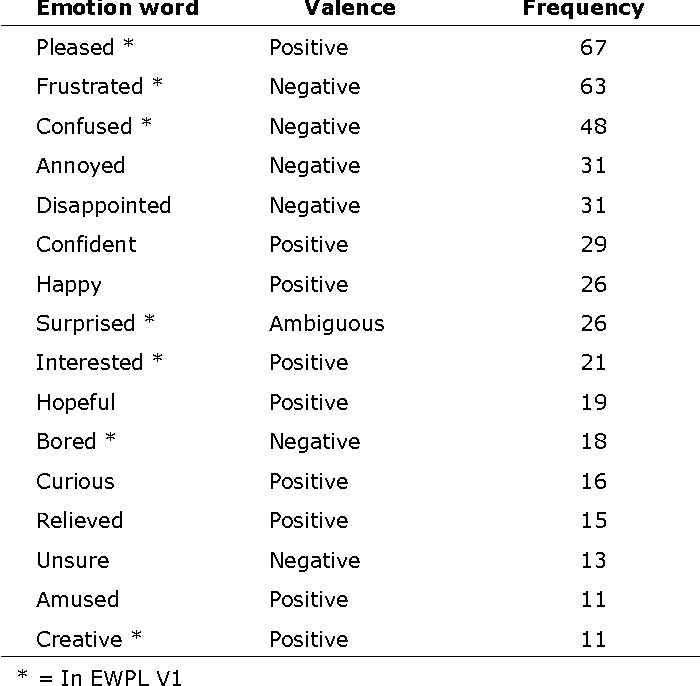
\includegraphics[width=0.5\textwidth]{pic-1.png}
  \caption{Measuring positive affective Frequency}
  \label{fig:example}
\end{figure}


\begin{figure}[h]
  \centering
  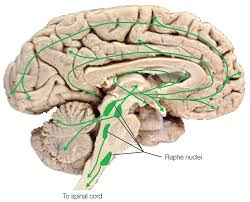
\includegraphics[width=0.5\textwidth]{pic-7.jpeg}
  \caption{Measuring positive affective reactions}
  \label{fig:example}
\end{figure}



\subsection{Subjective ratings of conscious pleasure}
By the term positive affect, almost everyone means a
conscious feeling of pleasure, a quintessentially subjective
phenomenon. Conscious pleasure is the only form of
pleasure of which many people can conceive. Take away
consciousness and for them you take away also the
meaning of pleasure, for they regard an unconscious
pleasure as a contradiction in terms (even if they allow
other implicit psychological processes such as unconscious memory, unconscious perception, etc.) This
tendency to define affective as necessarily meaning a
conscious feeling of pleasure/displeasure is exactly why
many have sometimes asserted that ‘‘affect can be studied
only in humans who can say what they feel.’’ The insistence on conscious feeling as the defining feature of affect
is understandable, but in my view mistaken.

\subsection{ Unspeakable ‘‘feelings’’: Unconscious core processes of affective reaction}

To suggest the possibility of unconscious affective
reactions as real psychological processes is not in any
way to diminish the crucial importance of conscious
feelings of pleasure. I fully concur with the reader who
believes that conscious pleasure has a special status and
interest for psychology and neuroscience, and deserves
special consideration on its own. But there are several
reasons why an affective neuroscience or hedonic psychology of pleasure would be wise not to restrict itself to
the study of subjective reports.
Implicit or unconscious affective psychological processes may sometimes occur in the mind and brain independent of conscious feelings (Berridge, 1999;
Damasio, 1999; LeDoux, 1996; Zajonc, 2000), just as
psychological processes of perception, learning, and
cognition can occur independent of any conscious
awareness of them (Kihlstrom, 1999). ‘‘Core processes’’
of implicit affective reaction that remain unconscious
can still be manifest in observable affective reactions
(Winkielman, Berridge, \& Wilbarger, 2000).
A core process view posits that conscious introspection lacks direct access to basic hedonic processes, just
as it lacks direct access to many cognitive processes.
Consciousness must interpret affective reactions cognitively into awareness just as it must interpret perception of other complex stimuli(Wilson, Lindsey, \& Schooler, 2000). The primary limitation of subjective reports of conscious pleasure is that they are
limited to just that—the subset of pleasurable feelings
that can be consciously accessed or even invented by
cognitive processes of representation and self-monitoring. Subjective reports may miss some positive affective
reactions that occur to an event without a person being
aware of that causal event . Further, in
a subset of those cases, the person might not even be
aware of having an affective reaction at all ((Winkielman, Zajonc, \& Schwarz, 1997).For example, a photograph of a happy facial expression that is presented
subliminally and masked may fail to produce any conscious report of affect or emotion or shift in hedonic
feelings at all, yet still increase a persons subsequent
behavioral consumption of a fruit drink and subjective
affective rating of it later(Winkielman, Zajonc, \& Schwarz, 1997). Conversely, a subliminally
presented angry face can reduce those subsequent reactions to the affect-laden drink, again without producing
any conscious emotion at the moment the face is
presented.
\begin{figure}[h]
  \centering
  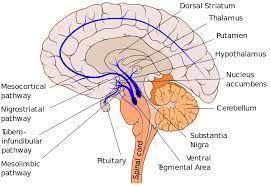
\includegraphics[width=0.5\textwidth]{pic-6.jpeg}
  \caption{Brain causation of positive affective reaction}
  \label{fig:example}
\end{figure}


\subsection{Behavioral and physiological measures of positive affective reaction}
Behavioral and physiological measures provide one
means of studying affective reactions whether or not a
conscious affective reaction is reported. Physiological
autonomic and brain imaging techniques provide other
potential measures. These measures can be applied to
animals as well as humans, which considerably extends
the range of opportunity available for probing the brain
mechanisms involved. The question of what an animal
feels is fascinating, though difficult, but the question of
how an animal reacts through behavioral and physiological responses to a positive affective event is as approachable and objectively answerable as the question
of how a person reacts. Such studies of animal reactions
have revealed useful insights into how brain systems
generate core liking reactions, and so will be an important focus.


\subsection{Diverse measures and concepts of positive affect in
animals}

Even affective neuroscientists who primarily study
positive affective reactions and reward in animals have
taken a spectrum of different approaches to measure
and understand positive affective reactions and their
K.C. Berridge / Brain and Cognition 52 (2003) 106–128 107
brain mechanisms. For example, Rolls takes an essentially behaviorist approach, identifying positive affective reaction or emotion with the occurrence of
behavioral response reinforcement (e.g., Rolls, 1999).
‘‘The essence of the proposal is that emotions are states
elicited by rewards and punishments, including changes
in rewards and punishments. A reward is anything for
which an animal will work. A punishment is anything
that an animal will work to escape or avoid’’ (Rolls,
1999, pp. 60–61). Thus for Rolls, positive emotion is
the state produced by any worked for reinforcer. This
approach defines the psychological process of positive
affect in terms of the behavioral event that caused it
(e.g., presentation of a worked-for reward). It does not
attempt to identify intrinsic psychological features of
positive affective reaction that distinguish it from other
psychological processes also elicited by the reinforcer,
such as learning. A behaviorist-reinforcement approach
has the advantage of simplicity and behavioral objectivity, but gives little insight into the affective nature of
emotion for those who wish to understand the psychology of pleasure. Defining positive emotion as reinforcement also encounters empirical difficulties (as
Rolls acknowledges) in certain cases where response
reinforcement learning is dissociated from other aspects
of positive emotion. For example, positive affective
reactions can occur in absence of behavioral reinforcement, in cases where no response is being trained.
Conversely, behavioral reinforcement can occur in absence of positive affective reaction, in cases where the
reinforcer removes an unpleasant state, or in other
cases where a manipulation directly strengthens stimulus-response associations or promotes other non-affective types of learning.



\subsection{ A prototype positive affective reaction: Hedonic reactions to sweet taste}


The facial expression of a human infant to a sweet
taste is one example of a behavioral positive affective
reaction to sensory pleasure (Steiner, Glaser, Hawilo, \& Berridge, 2001)
. Normal human infants have essentially just two patterns of facial expressions to tastes: positive affective versus negative affective
(Fig. 1). The sweet taste of sugar normally elicits positive affective patterns of lip smacking and rhythmic series of tongue protrusion movements. These are
accompanied by relaxation of the muscles of the middle
face, and on rare occasions, even a smile that can extend
to the full classic Duchenne type involving simultaneous



\begin{figure}[h]
  \centering
  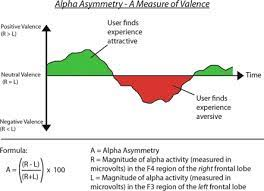
\includegraphics[width=0.5\textwidth]{pic-3.jpeg}
  \caption{MEASURES OF POSITIVE AFFECTIVE
REACTION}
  \label{fig:example}
\end{figure}





\section{Physiological measures of positive affective reaction}

Physiological reactions (e.g., EEG, galvanic skin response), brain imaging techniques (e.g., PET, fMRI),
and neuronal monitoring techniques (e.g., electrophysiological recording) provide another potentially exciting
means to objectively measure positive affective reactions
(Bechara, Damasio, Tranel, \& Damasio, 1997; Davidson \& Sutton, 1995; Fox \& Davidson, 1986; Larsen \& Fredrickson, 1999)
 Central measures of brain activation
have special potential to reveal positive affective reactions, and have been used to detect individual differences
in human affective reactions representing individual affective styles. Of course, the
difficult challenge is to identify which physiological or
neural reactions are reliable markers for positive affect
in particular (versus markers of other processes evoked
by the stimulus), but several promising ones have been
suggested (Bechara, Damasio, Tranel, \& Damasio, 1997; Davidson \& Sutton, 1995; Fox \& Davidson, 1986; Larsen \& Fredrickson, 1999)



\subsection{Conceptual issues for affective cognitive neuroscience: What does it mean to mediate pleasure?}


A major conceptual issue for the science of mindbrain relations concerns the idea that brain systems
mediate psychological functions such as positive affect.
On the surface ‘‘to mediate’’ seems clear enough, and is
commonly used without further definition. But the
concept actually has several possible meanings,
which can be mixed, leading to confusion. A better
112 K.C. Berridge / Brain and Cognition 52 (2003) 106–128
understanding of mind–brain relations can be gained by
keeping clear the different meanings  (Bechara, Damasio, Tranel, \& Damasio, 1997; Davidson \& Sutton, 1995; Fox \& Davidson, 1986; Larsen \& Fredrickson, 1999)


\subsection{Meanings of mediate: Neural consequence, sufficient cause, and/or necessary cause }

When cognitive, affective, or behavioral neuroscientists assert that a brain structure mediates a psychological process they generally mean one or more of three
things, which I will call neural marker, sufficient cause,
and necessary cause definitions. Often all three meanings
are meant simultaneously. But these meanings need not
and sometimes do not go together. So it is helpful to
consider the differences among these meanings before we
attempt to answer the question of which brain systems
mediate positive affective reactions.



\section{Brain causation of positive affective reaction}
Now we are ready to examine more closely which
brain systems actually cause positive affective reactions
to sensory pleasure, either as sufficient causes for super 
normal liking or necessary causes for normal pleasure.
We will consider specifically several brain systems that
are thought to be involved in positive affect: prefrontal
and cingulate cortex, the nucleus accumbens and its
mesolimbic projections, lateral hypothalamus and other
structures associated with brain stimulation reward, the
ventral pallidum, and the brainstem (especially the
parabrachial nucleus)

\begin{figure}[h]
  \centering
  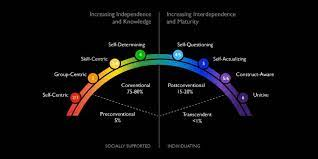
\includegraphics[width=0.5\textwidth]{pic-2.jpeg}
  \caption{Unspeakable “feelings”: Unconscious core processes of
affective reaction}
  \label{fig:example}
\end{figure}





\subsection{Consequence versus cause and generation versus use in action}
It seems clear that orbitofrontal cortex activation is a
good neural marker for positive affective reactions (as
well as for negative affective reactions). However, orbitofrontal status is less clear as a cause for generating
positive affective reactions. While there are a few reports
that rats will work to administer a microinjection of
cocaine or related drugs directly into their medial prefrontal cortex , there is little other evidence regarding
sufficient causation. And self-administration itself is
open to the question of whether the rats actually like as
well as want prefrontal microinjections, though it is at
least suggestive for a sufficient cause of positive affective
reaction. If so, such causation might be indirect rather
than direct. The prefrontal cortex projects massively to
the subcortical nucleus accumbens (Zahm, 2000), and
there is strong evidence that neurotransmission in accumbens can be a sufficient cause for positive affective. Orbitofrontal cortex might possibly regulate activation of positive affective reaction (Davidson, Jackson, & Kalin, 2000) via descending projections to causal
systems in accumbens, whether or not orbitofrontal
cortex directly generates positive affect itself.
There is less evidence that orbitofrontal cortex is a
necessary cause for a normal positive affective reaction.
Although a degree of apathy and lack of affect is
sometimes reported for human patients after damage to
the dorsomedial prefrontal cortex, the nearly opposite
symptoms of euphoria, impulsiveness, and general
emotional disinhibition are more often reported after And even
these changes may involve not so much a change in core
processes of positive affective reaction themselves, so
much as a more subtle change in how patients act upon
their emotions


\section*{ True brain substrates for core liking}

The nucleus accumbens lies at the front of the brain
beneath the neocortex. It is divided into two primary
divisions, shell and core. The shell is positioned a bit like
an elongated pastry pie shell with core as the pie filling.
The shell wraps around the bottom and the sides of the
core, as though it held the core within it. But the accumbens shell also has its own special psychological
functions. The shell is the only accumbens region shown
so far to directly cause increases in positive affective
. 
Activation of brain opioid circuitry in the nucleus accumbens shell seems to be a true sufficient cause for
liking.
In animal affective neuroscience studies, microinjection of a drug directly into the brain can be made
gently and painlessly through previously implanted
brain cannulae. The rat is totally anesthetized weeks
before the experiment so microinjection cannula can
be surgically placed into the accumbens. When the rat
recovers, the microinjection cannula provides a channel directly to the brain structure. If a microinjection
of a tiny droplet of a drug that mimics a neurotransmitter is made, it activates receptors for that
neurotransmitter specifically on nearby neurons.
Susana Pecina provided a demonstration that opioid 
neurons in the shell of the nucleus are a sufficient cause.
She showed that a microinjection of morphine into the
posterior shell of the nucleus accumbens caused the
sweet component of a bittersweet taste to elicit more
positive facial affective reactions from rats than it normally would. The sugar taste became more than ordinarily liked within minutes of morphine activation of
the opioid receptors in the nucleus accumbens shell.
Microinjections also caused the rats subsequently to
want to eat more of the food that they now liked
more.
In order to be sure that the opioid cause of positive
affective reactions was specifically in the shell of the
nucleus accumbens, Pecina mapped the precise borders ~
of the positive affect site using a technique based on Fos
plumes.Fos plumes are visible markers that show where
a drug microinjection activates receptors in the brain.
Visualizing Fos plumes is a bit like dripping food coloring into a glass of water, where drops form distinct
plumes for several moments before dispersing (Fig. 3).
When molecules of a drug or neurotransmitter activate
receptors on a neuron, a cascade of biochemical changes
triggered in the internal metabolic processes of the
neuron can cause activation of early intermediate
genes, such as c-fos. Gene activation of c-fos causes the
production of corresponding Fos protein inside the
neuron. Neurons with dense Fos protein can be seen by
treating slices of brain tissue with chemicals that causes
Fos to stain dark, and then examining the brain slice
under a microscope. A distinct Fos plume of stained
neurons can be identified on the brain slice (if processed
within an hour or so of the microinjection), which shows
where the drug microinjection triggered neurotransmitter receptors sufficiently to cause changes in neuronal
function.
When the opioid liking and wanting site was
mapped, it appeared restricted to the medial and posterior portion of the shell of the nucleus accumbens
(Pecina & Berridge, 2000). Thus the caudal region of the ~
shell of the nucleus accumbens seems to contain special
opioid neural circuits where morphine activation is a
sufficient cause of enhanced liking for food. This opioid-accumbens liking subsystem is embedded in larger
mesolimbic neural systems related to wanting for food
and other types of reward 
An opioid neural circuit in accumbens shell for taste
liking is consistent with earlier studies that showed
positive affective reactions to sweetness were enhanced
. The same opiate drugs tend to suppress
negative aversive reactions, such as, just as they suppress pain. Thus
opiate drugs shift all affective reactions to taste towards
a positive affective pole, making sweetness generally
more liked and bitterness less disliked. Conversely,
drugs that block opioid receptors make tastes less liked
in rat taste reactivity studies, and make humans rate sweetness and foods as less pleasant than normal.
\begin{figure}[h]
  \centering
  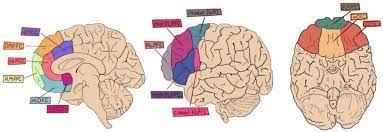
\includegraphics[width=0.5\textwidth]{pic-4.jpeg}
  \caption{TRUE BRAIN SUBSTRATES FOR CORE LIKING}
  \label{fig:example}
\end{figure}


\subsection{Circuits for feeling: Cortical connections with
accumbens core affect}

A core process view of emotion faces the challenge of
understanding how core liking is ever converted to
conscious pleasure. This would presumably require
secondary modulation of other brain systems that
causally mediate conscious feelings. There must be interaction between neural systems that generate consciousness and those that generate core processes of
emotion. Similar interaction might also sometimes occur
in the reverse direction, when core processes of emotion
are subject to voluntary regulation by cognitive systems
(Davidson et al., 2000). How could a core process for
positive affective reaction, caused in the nucleus accumbens shell, interact with cortical brain systems for
cognitive representation?
Pathways exist to relay a core process of positive
affect in accumbens shell to affective cortical systems
in just a few synapses, and so perhaps to create conscious pleasure feelings (Fig. 3). By one path, neurons
in nucleus accumbens shell project to a deep subcortical forebrain site directly behind the accumbens,
namely, the ventral pallidum (especially its medial
portion), which in turn projects to the mediodorsal
nucleus in the thalamus, which finally projects directly
to the prefrontal cortex regions that have been implicated in higher affective reactions.Thalamic mediodorsal relays also project to insular
cortex, which processes taste sensations and related
affect and cognition. This provides one potential way
for an opioid-induced activation of hedonic liking in
the accumbens shell to influence feelings of pleasure
that might be instantiated by limbic regions of neocortex.

\begin{figure}[h]
  \centering
  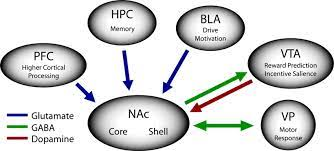
\includegraphics[width=0.5\textwidth]{pic-8.jpeg}
  \caption{ortical connections with accumbens
core affec}
  \label{fig:example}
\end{figure}




\subsubsection{Second sufficient cause for positive affective reactions: Hindbrain parabrachial nucleus}


idespread brain systems. Core processes of positive
affective reaction are not localized to a single brain site,
but distributed in neural circuits that stretch across the
brain. The nucleus accumbens shell is not the only brain
site able to cause increased positive affective reactions to
an event. Recent studies have identified another neurotransmitter circuit in another part of the rat brain
equally able to cause enhanced positive affective reactions to a sweet taste: namely, a benzodiazepine/GABA
circuit in the parabrachial nucleus of the hindbrain.
It was a bit of a surprise that benzodiazepine drugs
can enhance liking for a sensory pleasure, because
those drugs are much better known for their strong
sedative and anxiety reduction effects (Cooper, Higgs, \& Clifton, 1995) brain, and do different things at each place. Anxiety
reduction may be mediated in part by forebrain strucK.C. Berridge / Brain and Cognition 52 (2003) 106–128 121
tures, whereas positive affective effects of benzodiaze pines occur in the hindbrain. It is now well documented
that benzodiazepine drugs, such as diazepam or mi, cause animals to eat large quantities of food , and can cause humans to
overeat too. Cooper proposed nearly 20 years ago that benzodiaze pine enhancements of food wanting might be mediated
by enhancement of liking or positive reaction to the
hedonic impact of a taste. There
is now robust evidence to support his suggestion that
this wanting reflects liking.



\section{Pleasure: One brain circuit or many?}

How many types of pleasure are there in the brain?
Does one brain circuit mediate a core process of
liking shared by all types of pleasure? Or does each
type of pleasure have its own core process and neural
substrate? This is a question that has hardly begun to
be asked in experimental studies, let alone to be answered. However there is at least evidence to suggest
that several basic types of sensory pleasure, including
food pleasure, drug pleasure, and sex pleasure, all
share in common at least certain stages of their neural
circuits.
Fig. 4. Site within ventral pallidum that is a necessary cause for normal positive affective reactions to sweet tastes (A). Excitotoxin lesions in the
ventral pallidum (black zone) cause rats to respond with negative aversive reaction even to sweet tastes that are normally palatable—as though it
made them bitter. Larger grey zone represents the adjacent lateral hypothalamu. Brainstem parabrachial nucleus in the
pons where microinjection of benzodiazepine causes increased positive reactions to a sweet taste (B)(modified from Pecina \& Berridge, 2000). ~
Sideways views in A and B show anterior–posterior position of the section in the rat brain, and position of the equivalent structures in human brain.
K.C. Berridge / Brain and Cognition 52 (2003) 106–128 123
Parts of the mesolimbic reward system, involving the
nucleus accumbens shell (opioid system) and its projections to ventral pallidum, are especially good can to cause liking for multiple types of basic
sensory pleasure. Many studies have also indicated the
mesolimbic dopamine projection to this system to be a
shared substrate at least for wanting (though probably
not for liking) for multiple types of reward, including
food, sex, heroin, cocaine and related drugs, rewarding
electrical brain stimulation, maternal interaction with
infants, and even social and culturally based rewards
(e.g., money and videogames for humans)(Berridge \& Robinson, 1998; Depue \& Collins, 1999; Everitt, 1990; Fiorino, Coury, \& Phillips, 1997; Mermelstein \& Becker, 1995; Panksepp, 1998; Shizgal, 1999; Thut et al., 1997; Wise, 1998)
. Future studies may clarify the precise role of components within this system in liking
versus wanting, in relating those core processes to
each other, or in other roles regarding basic sensory
pleasures.
Also to be explored are the brain bases of more abstract forms of positive affect, including social joy, love,
intellectual pleasures, aesthetic appreciation, and moral
appreciation. Do such elevated positive emotions share
neural underpinnings with sensory liking? That remains
to be seen. The search for understanding of how positive
affective reactions are generated by the brain will long
remain a source of cerebral pleasure for those who have
a taste for that sort of thing


\begin{figure}[h]
  \centering
  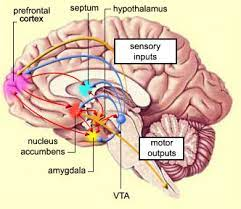
\includegraphics[width=0.5\textwidth]{pic-5.jpeg}
  \caption{PLEASURE: ONE BRAIN CIRCUIT OR MANY?}
  \label{fig:example}
\end{figure}

\newpage


\section{Conclusion}
Positive affective reactions provide a window into
how the brain generates positive affect. Even when affective reactions are not directly read out into conscious
awareness, core processes of affect and motivation may
nonetheless be manifest as positive affective reactions.
Behavioral affective reactions to taste have allowed
progress in identifying how the brain causally mediates
core processes of positive affect. Subsystems of the nucleus accumbens shell, the ventral pallidum, and brainstem nuclei play a special role in causing liking in the
brain. The relation of core processes to conscious pleasure, the role of particular subcomponents, and the relation among multiple types of positive affective reaction
continue to be exciting topics for research on pleasures
of the brain.



\section{Acknowledgments}

I am grateful to Dr. Jaak Panksepp, Sheila Reynolds,
Dr. Louis Schmidt, Dr. Jay Schulkin, Dr. Peter Shizgal,
and Dr. Elliot Valenstein for helpful comments on earlier versions of the manuscript.




\section*{References}

\begin{enumerate}
   \bibitem{balleine1998}
Balleine, B. W., \& Dickinson, A. (1998). Goal-directed instrumental action: Contingency and incentive learning and their cortical substrates. \textit{Neuropharmacology}, 37(4--5), 407--419.

\bibitem{bassareo1997}
Bassareo, V., \& DiChiara, G. (1997). Differential influence of associative and nonassociative learning mechanisms on the responsiveness of prefrontal and accumbal dopamine transmission to food stimuli in rats fed ad libitum. \textit{Journal of Neuroscience}, 17(2), 851--861.

\bibitem{baumeister2000}
Baumeister, A. A. (2000). The Tulane Electrical Brain Stimulation Program: A historical case study in medical ethics. \textit{Journal of the History of the Neurosciences}, 9(3), 262--278.

\bibitem{baxter2000}
Baxter, M. G., Parker, A., Lindner, C. C., Izquierdo, A. D., \& Murray, E. A. (2000). Control of response selection by reinforcer value requires interaction of amygdala and orbital prefrontal cortex. \textit{Journal of Neuroscience}, 20(11), 4311--4319.

\bibitem{bechara2000}
Bechara, A., Damasio, H., \& Damasio, A. R. (2000). Emotion, decision making, and the orbitofrontal cortex. \textit{Cerebral Cortex}, 10(3), 295--307.

\bibitem{bechara1997}
Bechara, A., Damasio, H., Tranel, D., \& Damasio, A. R. (1997). Deciding advantageously before knowing the advantageous strategy. \textit{Science}, 275(5304), 1293--1295.

\end{enumerate}

\end{document}


\end{document}